\documentclass{beamer}
\usepackage[utf8]{inputenc}

\usetheme{Boadilla}
\usecolortheme{lily}
\usepackage{amsmath,amssymb,amsfonts,amsthm}
\usepackage{mathtools}
\usepackage{txfonts}
\usepackage{tkz-euclide}
\usepackage{listings}
\usepackage{adjustbox}
\usepackage{array}
\usepackage{tabularx}
\usepackage{lmodern}
\usepackage{circuitikz}
\usepackage{tikz}
\usepackage{graphicx}

\setbeamertemplate{footline}
{
  \leavevmode%
  \hbox{%
  \begin{beamercolorbox}[wd=\paperwidth,ht=2.25ex,dp=1ex,right]{author in head/foot}%
    \insertframenumber{} / \inserttotalframenumber\hspace*{2ex} 
  \end{beamercolorbox}}%
  \vskip0pt%
}

\usepackage{tcolorbox}
\tcbuselibrary{minted,breakable,xparse,skins}




\providecommand{\nCr}[2]{\,^{#1}C_{#2}} % nCr
\providecommand{\nPr}[2]{\,^{#1}P_{#2}} % nPr
\providecommand{\mbf}{\mathbf}
\providecommand{\pr}[1]{\ensuremath{\Pr\left(#1\right)}}
\providecommand{\qfunc}[1]{\ensuremath{Q\left(#1\right)}}
\providecommand{\sbrak}[1]{\ensuremath{{}\left[#1\right]}}
\providecommand{\lsbrak}[1]{\ensuremath{{}\left[#1\right.}}
\providecommand{\rsbrak}[1]{\ensuremath{{}\left.#1\right]}}
\providecommand{\brak}[1]{\ensuremath{\left(#1\right)}}
\providecommand{\lbrak}[1]{\ensuremath{\left(#1\right.}}
\providecommand{\rbrak}[1]{\ensuremath{\left.#1\right)}}
\providecommand{\cbrak}[1]{\ensuremath{\left\{#1\right\}}}
\providecommand{\lcbrak}[1]{\ensuremath{\left\{#1\right.}}
\providecommand{\rcbrak}[1]{\ensuremath{\left.#1\right\}}}
\theoremstyle{remark}
\newtheorem{rem}{Remark}
\newcommand{\sgn}{\mathop{\mathrm{sgn}}}
\providecommand{\abs}[1]{\left\vert#1\right\vert}
\providecommand{\res}[1]{\Res\displaylimits_{#1}} 
\providecommand{\norm}[1]{\lVert#1\rVert}
\providecommand{\mtx}[1]{\mathbf{#1}}
\providecommand{\mean}[1]{E\left[ #1 \right]}
\providecommand{\fourier}{\overset{\mathcal{F}}{ \rightleftharpoons}}
%\providecommand{\hilbert}{\overset{\mathcal{H}}{ \rightleftharpoons}}
\providecommand{\system}{\overset{\mathcal{H}}{ \longleftrightarrow}}
	%\newcommand{\solution}[2]{\textbf{Solution:}{#1}}
%\newcommand{\solution}{\noindent \textbf{Solution: }}
\providecommand{\dec}[2]{\ensuremath{\overset{#1}{\underset{#2}{\gtrless}}}}
\newcommand{\myvec}[1]{\ensuremath{\begin{pmatrix}#1\end{pmatrix}}}
\let\vec\mathbf

\lstset{
%language=C,
frame=single, 
breaklines=true,
columns=fullflexible
}

\numberwithin{equation}{section}

\lstset{
  language=Python,
  basicstyle=\ttfamily\small,
  keywordstyle=\color{blue},
  stringstyle=\color{orange},
  numbers=left,
  numberstyle=\tiny\color{gray},
  breaklines=true,
  showstringspaces=false
}

\title{Problem 2.10.52}
\author{ee25btech11023-Venkata Sai}

\date{\today} 
\begin{document}

\begin{frame}
\titlepage
\end{frame}

\section*{Outline}
\begin{frame}
\tableofcontents
\end{frame}

\section{Problem}

\begin{frame}
\frametitle{Problem}
Let $\vec{a} = \hat{\vec{i}} + 2\hat{\vec{j}} + \hat{\vec{k}}$, $\vec{b} = \hat{\vec{i}} - \hat{\vec{j}} + \hat{\vec{k}}$ and $\vec{c} = \hat{\vec{i}} + \hat{\vec{j}} - \hat{\vec{k}}$. A vector in the plane of $\vec{a}$ and $\vec{b}$ whose projection on $\vec{c}$ is $\frac{1}{\sqrt{3}}$, is 
\begin{enumerate}
\item 4$\hat{\vec{i}} - \hat{\vec{j}} + 4\hat{\vec{k}}$
\item 3$\hat{\vec{i}} + \hat{\vec{j}} - 3\hat{\vec{k}}$
\item $2\hat{\vec{i}} + \hat{\vec{j}} - 2\hat{\vec{k}}$
\item $4\hat{\vec{i}} + \hat{\vec{j}} - 4\hat{\vec{k}}$
\end{enumerate}
\end{frame}
%\subsection{Literature}
\section{Solution}
 
\subsection{Coplanarity}
\begin{frame}
\setcounter{section}{1}
\frametitle{Coplanarity}
Given $\vec{a}=\myvec{1\\2\\1},\vec{b}=\myvec{1\\-1\\1},\vec{c}=\myvec{1\\1\\-1}$ \\

Let $\vec{r}$ be coplanar to $\vec{a}$ and $\vec{b}$
\begin{align}
 \vec{r}=\vec{a}+t\vec{b} 
 \end{align}
\end{frame}
\subsection{Simplify}
\begin{frame}
\frametitle{Simplify}
Given the projection of $\vec{r}$ on $\vec{c}$ is $\frac{1}{\sqrt{3}}$
\begin{align}
\frac{|\vec{r}^\top\vec{c}|}{\norm{\vec{c}}} = \frac{1}{\sqrt{3}} 
\end{align}
\begin{align}
\vec{r}^\top\vec{c}&=\brak{\vec{a}+t\vec{b}}^\top\vec{c}\\
&=\brak{\vec{a}^\top+t\vec{b}^\top}c \\
&=\vec{a}^\top\vec{c}+t\brak{\vec{b}^\top\vec{c}} 
\end{align}
\begin{align}
\vec{r}^\top\vec{c}-\vec{a}^\top\vec{c}=t\brak{\vec{b}^\top\vec{c}}  \\
\implies t=\frac{\vec{r}^\top\vec{c}-\vec{a}^\top\vec{c}}{\vec{b}^\top\vec{c}}
\end{align}
\end{frame}
\subsection{Finding Values}
\begin{frame}
\frametitle{Finding Values}
\begin{align}
    \vec{r}=\vec{a}+\brak{\frac{\vec{r}^\top\vec{c}-\vec{a}^\top\vec{c}}{\vec{b}^\top\vec{c}}}\vec{b} \\
    \vec{r}=\vec{a}+\brak{\frac{\pm\frac{\norm{\vec{c}}}{\sqrt{3}}-\vec{a}^\top\vec{c}}{\vec{b}^\top\vec{c}}}\vec{b}
\end{align}
\begin{align}
\norm{\vec{c}}^2=\vec{c}^\top\vec{c}&=\myvec{1&1&-1}\myvec{1\\1\\-1} \\
&=1+1+1=3  \implies \norm{\vec{c}}=\sqrt{3}
\end{align} 
\begin{align}
\vec{a}^\top\vec{c}=\myvec{1&2&1}\myvec{1\\1\\-1}=1+2-1=2 
\end{align}
\end{frame}
\subsection{Conclusion}
\begin{frame}
\frametitle{Conclusion}
\begin{align}
\vec{b}^\top\vec{c}=\myvec{1&-1&1}\myvec{1\\1\\-1}=1-1-1=-1
\end{align}
\begin{align}
\vec{r}=\myvec{1\\2\\1}+\brak{\frac{\pm1-2}{-1}}\myvec{1\\-1\\1} 
\end{align}
\begin{align}
\implies \vec{r}=\myvec{1\\2\\1}+\myvec{1\\-1\\1}\ \text{or}\ \myvec{1\\2\\1}+3\myvec{1\\-1\\1}
\implies \vec{r}=\myvec{2\\1\\2}\ \text{or} \myvec{4\\-1\\4}
\end{align}
Hence Option(1) is the correct answer
\end{frame}

\subsection{Plot}
\begin{frame}[fragile]
\frametitle{Plot}

\begin{figure}[h!]
   \centering
   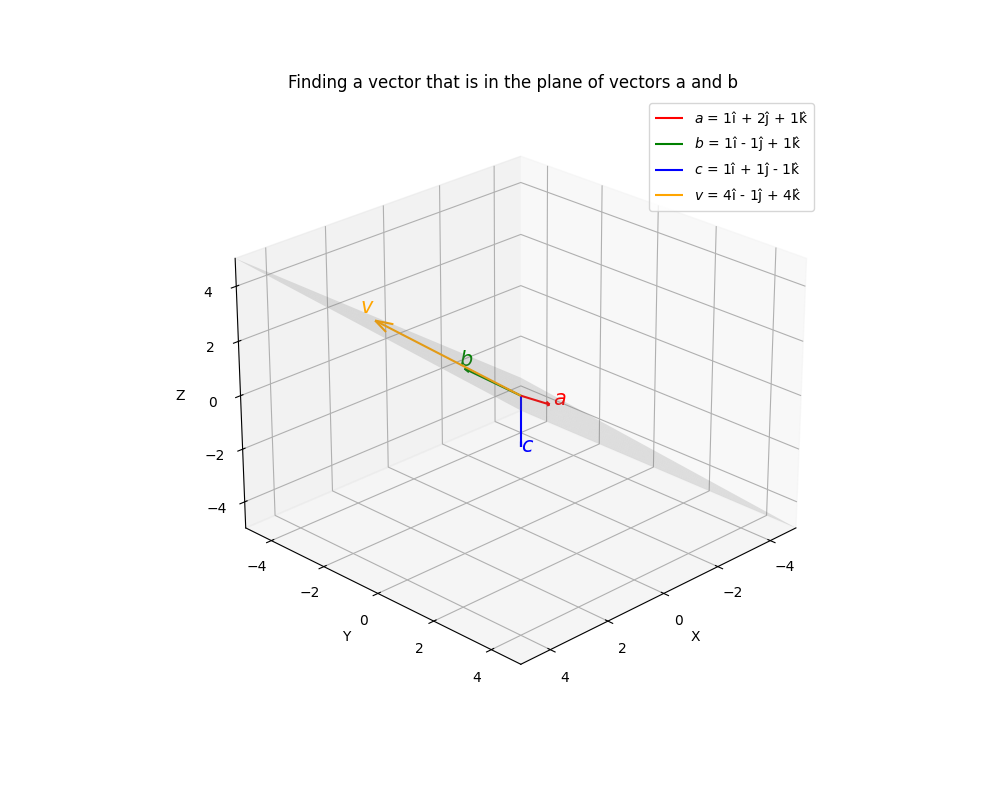
\includegraphics[width=0.7\columnwidth]{figs/fig1.png}
	\caption{}
   \label{}
\end{figure}
\end{frame}

\section{C Code}
\begin{frame}[fragile]
\frametitle{C Code}
\begin{lstlisting}[language=C]
void get_vectors(double* vector_data) {
    vector_data[0] = 1.0; vector_data[1] = 2.0; vector_data[2] = 1.0;
    vector_data[3] = 1.0; vector_data[4] = -1.0; vector_data[5] = 1.0;
    vector_data[6] = 1.0; vector_data[7] = 1.0; vector_data[8] = -1.0;
    vector_data[9] = 4.0; vector_data[10] = -1.0; vector_data[11] = 4.0;
}
    \end{lstlisting}
\end{frame}
\section{Python Code}
\begin{frame}[fragile]
\frametitle{Calling C Function}
\begin{lstlisting}[language=Python]
import ctypes
import numpy as np

def load_vectors_from_c():

    # Load the shared C library. Assumes the file exists.
    lib = ctypes.CDLL('./plane.so')

    double_array_12=ctypes.c_double*12
    out_vectors=double_array_12()
    lib.get_vectors.argtypes=[ctypes.POINTER(ctypes.c_double)]
    lib.get_vectors(out_vectors)
    # Reshape the data and return the individual vectors
    out_vector = np.array(out_vectors).reshape(4, 3)
    a, b, c, v = out_vector[0], out_vector[1], out_vector[2], out_vector[3]
    return a, b, c, v
\end{lstlisting}
\end{frame}

\begin{frame}[fragile]
\frametitle{Python Code for Plotting}
\begin{lstlisting}[language=Python]
#Code by GVV Sharma
#September 12, 2023
#Revised July 21, 2024
#released under GNU GPL

import sys
import matplotlib.pyplot as plt
import numpy as np
sys.path.insert(0, '/workspaces/urban-potato/matgeo/codes/CoordGeo/') 
from call import load_vectors_from_c
hat_symbol = '\u0302'
from line.funcs import *
from triangle.funcs import *
from conics.funcs import circ_gen

a, b, c, v = load_vectors_from_c()
 
\end{lstlisting}
\end{frame}

\begin{frame}[fragile]
\frametitle{Python Code for Plotting}
\begin{lstlisting}[language=Python]
vectors = [a, b, c, v]
colors = ['r', 'g', 'b', 'orange']
labels = ['a', 'b', 'c', 'v']
def format_original_label(name, vec):
    x, y, z = int(vec[0]), int(vec[1]), int(vec[2])
    y_part = f"+ {y}ĵ" if y >= 0 else f"- {abs(y)}ĵ"
    z_part = f"+ {z}k̂" if z >= 0 else f"- {abs(z)}k̂"
    return f'${name}$ = {x}î {y_part} {z_part}'

# Create a 3D plot
fig = plt.figure(figsize=(10, 8))
ax = fig.add_subplot(111, projection='3d')
origin = [0, 0, 0]

# Plot vectors
 for vec, color, name in zip(vectors, colors, labels):
    legend_label = format_original_label(name, vec)
    ax.quiver(*origin, *vec, color=color,arrow_length_ratio=0.1, label=legend_label)
\end{lstlisting}
\end{frame}

\begin{frame}[fragile]
\frametitle{Python Code for Plotting}
\begin{lstlisting}[language=Python]
    ax.text(*(vec * 1.1), f'${name}$', color=color, fontsize=15)
x_plane = np.linspace(-5, 5, 10)
y_plane = np.linspace(-5, 5, 10)
X, Y = np.meshgrid(x_plane, y_plane)
Z = X
ax.plot_surface(X, Y, Z, alpha=0.2, color='gray')
ax.set_xlabel('X')
ax.set_ylabel('Y')
ax.set_zlabel('Z')
ax.set_title('Finding a vector that is in the plane of vectors a and b')
ax.legend()
ax.grid(True)
plt.show()
plt.savefig('fig.png')
\end{lstlisting}
\end{frame}

\end{document}
